\documentclass[10pt,a4paper]{article}
\usepackage[T1]{fontenc}
\usepackage[utf8]{inputenc}
\usepackage[english]{babel}
\usepackage{amsmath}
\usepackage{amsfonts}
\usepackage{amssymb}
\usepackage{graphicx}
\usepackage{caption}
\usepackage{subcaption}
\usepackage{algpseudocode}
\usepackage{algorithm}


\author{Joan Puigcerver i Pérez\\
\begin{footnotesize}
\textit{joapuipe@upv.es}
\end{footnotesize}}
\title{A Genetic Algorithm for the Job-Shop Scheduling Problem}
\begin{document}
\maketitle
\section{Introduction}
The job-shop scheduling problem (JSP) consists on a given set of $n$ jobs to perform $\mathcal{J} = \{J_1, \ldots, J_n\}$. Each job $j$ is composed by $t$ tasks $\mathcal{T}_j = <\theta_{j,1}, \ldots, \theta_{j,t}>$ ($1 \leq j \leq n$), each of them with an associated duration $D_{j,k}$ ($1 \leq j \leq n$, $1 \leq k \leq t$). Each task $\theta_{j,k}$ needs also an specific resource $r_{j,k} \in \mathcal{R}$ from the set of $m$ resources $\mathcal{R} = \{R_1, \ldots, R_m\}$, $(1 \leq j \leq n, 1 \leq k \leq t)$. The objective is to schedule the start time $S_{j,k}$ of each task $\theta_{j,k}$ to minimize the completion time of the whole set of jobs (the timespan). This has to be done subject to the following restrictions: all tasks within a job have to be completed sequentially and no two tasks are assigned to the same machine at the same time. This two restrictions can be formally specified using the bellow equations.

\begin{eqnarray}
S_{j,k} \geq S_{j,k-1} + D_{j,k-1} : 1 \leq j \leq n, 2 \leq k \leq t \label{eq:consecutive_tasks} \\
r_{j,k} \neq r_{j,k'} \vee S_{j,k} \notin  [S_{j,k'}, S_{j,k'} + D_{j,k'}] : 1 \leq j \leq n, 1 \leq k,k' \leq t, k \neq k' \label{eq:single_core_machines}
\end{eqnarray}

These two restrictions, as stated in the previous equations, imply an additional restriction: once a task starts, it cannot be preempted by any other task.\\

It has been proven that this problem is NP-Hard and can be reduced to finding the minimum cost Hamiltonian path in a directed graph with weighted edges (a disjunctive graph)\cite{lenstra1977complexity,lenstra1979computational,blazewicz2000disjunctive}. Because of the complexity of the problem, exact solutions for big instances cannot be computed in a reasonable amount of time. Different approximate solutions based on branch and bound\cite{carlier1989algorithm}, simulated annealing\cite{van1992job}, genetic algorithms\cite{davis1985job}, and other techniques have been explored in the literature. Here we present a genetic algorithm (GA) that is able to produce reasonable solutions with a polynomial time complexity.

\section{Genetic Algorithm}
Genetic Algorithms are iterative algorithms that encode a solution for a given problem as an individual of a fixed-size population. At any given iteration, two or more individuals (solutions) are combined to create new individuals (this is called a crossover). Individuals may also be modified with random modifications of the encoded solution (mutations). The key process here is that individuals are combined and modified randomly and all of them are evaluated using a fitness function that has to be minimized (or maximized, depending on the problem). Then, only the best individuals from each iteration will survive to the next iteration (additionally, some ``bad'' solutions may survive which sometimes helps to avoid local optima).\\

Thus, in order to solve any optimization problem using GAs one must define how the solutions are encoded as individuals of the population, which fitness function has to be optimized, and how they are combined (crossover operation) and mutated (mutation operation) to create new individuals.

\subsection{Solution encoding}
A solution for a JSP instance can be represented as a direct acyclic graph (DAG) where each node represents a task and edges represent dependencies among tasks (the within-job task ordering and the resources dependencies). Then, the timespan is given by the longest path from the start node to the end node. The start node is defined as a dummy task called $\theta_I$ which takes 0 time steps and has an outgoing edge to the first task of each job $\theta_{j,1}, 1 \leq j \leq n$. The target node $\theta_F$ has incoming edges from the final task of each job $\theta_{j,t}, 1 \leq j \leq n$ and takes also 0 time steps to complete.\\

We use a typical representation for the JSP which encodes the restriction stated in equation \ref{eq:consecutive_tasks} implicitly (tasks within a job must be completed sequentially). The individuals encode a topological ordering of the DAG representing the solution. The tasks are represented only by their job identifier, and the task identifier is represented implicitly by the relative position of each task in the chromosome (for example, the first task from job 1, will be task 1, the second task from job 2 will be task 2, and so on). This allows us to represent the previous restriction implicitly in the chromosome. For instance, suppose the instance of the JSP represented in table \ref{tab:example_instance} with two jobs, two tasks for each job and two machines.\\

\begin{table}[h]
\centering
\begin{tabular}{|c|c|c|c|c|}
\hline 
& $\theta_{1,1}$ & $\theta_{1,2}$ & $\theta_{2,1}$ & $\theta_{2,2}$ \\
\hline
$r_{i,j}$ & 1 & 2 & 2 & 1 \\
$D_{i,j}$ & 3 & 2 & 5 & 1 \\
\hline
\end{tabular}
\caption{A JSP instance example for two jobs, two tasks for each job and two machines.}
\label{tab:example_instance}
\end{table}

The previous instance can be represented using the directed graph shown in figure \ref{fig:example_instance} and a possible solution would be the one depicted in figure \ref{fig:example_instance_sol}. The presented solution schedules $\theta_{1,1}$ before $\theta_{2,2}$ and $\theta_{2,1}$ before $\theta_{1,2}$. Tasks $\theta_{1,1}$ and $\theta_{2,1}$ can be done in parallel, same as tasks $\theta_{1,2}$ and $\theta_{2,2}$.\\

\begin{figure}[h]
\centering
\begin{subfigure}[b]{0.48\textwidth}
\centering
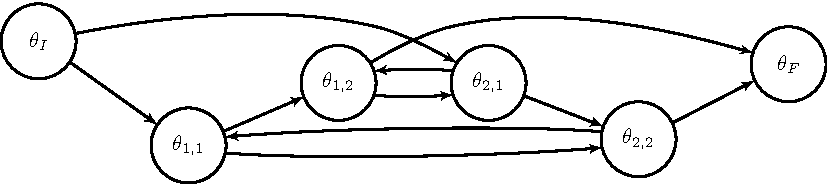
\includegraphics[width=\textwidth]{example_instance.pdf}
\caption{Directed graph representing the JSP instance from table \ref{tab:example_instance}.}
\label{fig:example_instance}
\end{subfigure}
~
\begin{subfigure}[b]{0.48\textwidth}
\centering
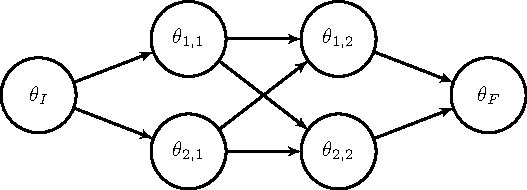
\includegraphics[width=\textwidth]{example_instance_sol.pdf}
\caption{A possible solution for the instance presented from table \ref{tab:example_instance}. }
\label{fig:example_instance_sol}
\end{subfigure}
\caption{}
\end{figure}

Note that, in the general case, multiple topological orderings can be obtained from a given DAG. Given \ref{fig:example_instance_sol}, table \ref{tab:example_instance_sols} shows four topological orderings of the same DAG which lead to four different representations of the same solution.

\begin{table}[h]
\centering
\begin{tabular}{|cccccc|cccc|}
\hline
\multicolumn{6}{|c|}{Topological ordering} & \multicolumn{4}{|c|}{Individual}\\
\hline
$\theta_I$ & $\theta_{1,1}$ & $\theta_{2,1}$ & $\theta_{1,2}$ & $\theta_{2,2}$ & $\theta_F$ & 1 & 2 & 1 & 2 \\
\hline
$\theta_I$ & $\theta_{2,1}$ & $\theta_{1,1}$ & $\theta_{2,2}$ & $\theta_{1,2}$ & $\theta_F$ & 2 & 1 & 2 & 1 \\
\hline
$\theta_I$ & $\theta_{1,1}$ & $\theta_{2,1}$ & $\theta_{2,2}$ & $\theta_{1,2}$ & $\theta_F$ & 1 & 2 & 2 & 1 \\
\hline
$\theta_I$ & $\theta_{2,1}$ & $\theta_{1,1}$ & $\theta_{1,2}$ & $\theta_{2,2}$ & $\theta_F$ & 2 & 1 & 1 & 2\\
\hline
\end{tabular}
\caption{The four possible topological orderings from the solution represent by figure \ref{fig:example_instance_sol} and their corresponding representation in the GA.}
\label{tab:example_instance_sols}
\end{table}

The DAG can be reconstructed from a topological ordering, given the definition of the instance. The direct approach that is used in our algorithm does this step with a worst-case cost of $O(n^2 t^2) = O(|\mathcal{T}|^2)$. Some data structures can be used to reduce this time complexity.

\subsection{Fitness function}
Since our objective is to minimize the timespan of the job-shop scheduling, we use this function as the fitness function to minimize by the genetic algorithm. Once the DAG representing the solution is obtained, the computation of the fitness function can be done by computing the longest path from $\theta_I$ to $\theta_F$ in the DAG. This is done in $O(|E|)$ using a dynamic programming scheme, where $E$ is the set of edges in the solution DAG.

\subsection{Crossover and mutation operations}
The used crossover algorithm is a generalization of the order crossover operator (OX) and was presented in \cite{bierwirth1995generalized}. A random pair of individuals of the population at some iteration are merged with probability $P_c$ to form a new individual. The crossover operation uses a random segment of the first parent as an implant that will be inserted in a random position in the chromosome of the second parent. Once the new elements have been implanted into the vector, the old-duplicated elements are removed. In order to create two individuals from the two parents, first one of the parents is used to extract the implant and then, the other parent is used.\\

When a new individual is created from a crossover, two random elements of the chromosome are swapped with probability $P_m$. The parents are not mutated to avoid the loss of the best solution found so far. 

\section{Experiments}
Different experiments were done using several instances of the JSP. Two types of instances were used: small and large instances. All small instances have 3 jobs that are characterized by the number of machines $m$ (3, 5 or 7), the number of tasks per job $t$ (5, 7 or 10) and the maximum value of the duration time $D_{max}$ (10, 50 or 100). A set of 10 instances are used for each combination of the three variables. All of the large instances are characterized have 3 jobs and 3 machines and are characterized by the variables $t$ (20, 25, 30) and $D_{max}$ (50, 100, 200). Also 10 instances are used for each combination of parameters.\\

In order to explore the effect of the parameters of the GA (population size, number of iterations, crossover probability and mutation probability), the small instances were used to measure the percentage of solutions proposed by the GA with a timespan greater than the reference solution (the lower this percentage is, the better). Additionally, the difference between the reference timespan for each instance (obtained with a commercial product) and the timespan of the solution found by the proposed genetic algorithm: $T_{ref} - T_{GA}$. The bigger the difference is, the better the proposed genetic algorithm is in comparison to the reference. If the reference is the exact solution to the JSP instance, the difference can be, at most 0.\\

Figure \ref{fig:evol_m_diff} shows the evolution of $T_{ref} - T_{GA}$ for different values of the mutation probability $P_m$. It is shown that there are no significant differences among many of the $P_m$ values. The better performance was achieved for $P_m = 0.1$. The population size for this experiments was set to 50, the number of iterations was also set to 50 and the crossover probability was set to 0.5. Intervals are shown for a 95\% confidence.\\

Figure \ref{fig:evol_c_diff} shows the evolution of $T_{ref} - T_{GA}$ for different values of the crossover probability $P_m$. The mutation probability was set to 0.1 and the rest of parameters were set as before. Here it is shown that the impact of the crossover probability is very significant, achieving the best performance when $P_c = 1$.\\

Figures \ref{fig:evol_pop_it_diff} and \ref{fig:evol_pop_it_worse} show the evolution of $T_{ref} - T_{GA}$ and $P(T_{GA} > T_{ref})$ for different values of the population size and number of iterations. This two functions are plot together because at some value of the $x$ coordinate, the expected number of generated individuals is the same in both scenarios. This expected number generated individuals is $O(P_c \cdot N \cdot I)$, where $N$ is the population size and $I$ is the number of iterations. In the experiment where the number of iterations was explored, the population size was set constant to 50, while when the explored variable was the population size, the number of iterations was 50. In both cases, the crossover probability was set to 0.5 and the mutation probability was set to 0.1. So, the cases where $Population = 500$ and $Iterations = 500$, the expected number of generated individuals is $0.5 \cdot 500 \cdot 50 = 12500$. These plots show that given a fixed number of expected individuals, it is better to have more iterations instead of a bigger population size. Notice that the confidence intervals for the $T_{ref} - T_{GA}$ curves do not overlap, so the differences are statistically significant (95\%). It is also shown that as we increase the value of these parameters, the quality of the obtained solution improves (and also the computation time required to obtain it).

\begin{figure}[h]
\centering
\begin{subfigure}[b]{0.45\textwidth}
\centering
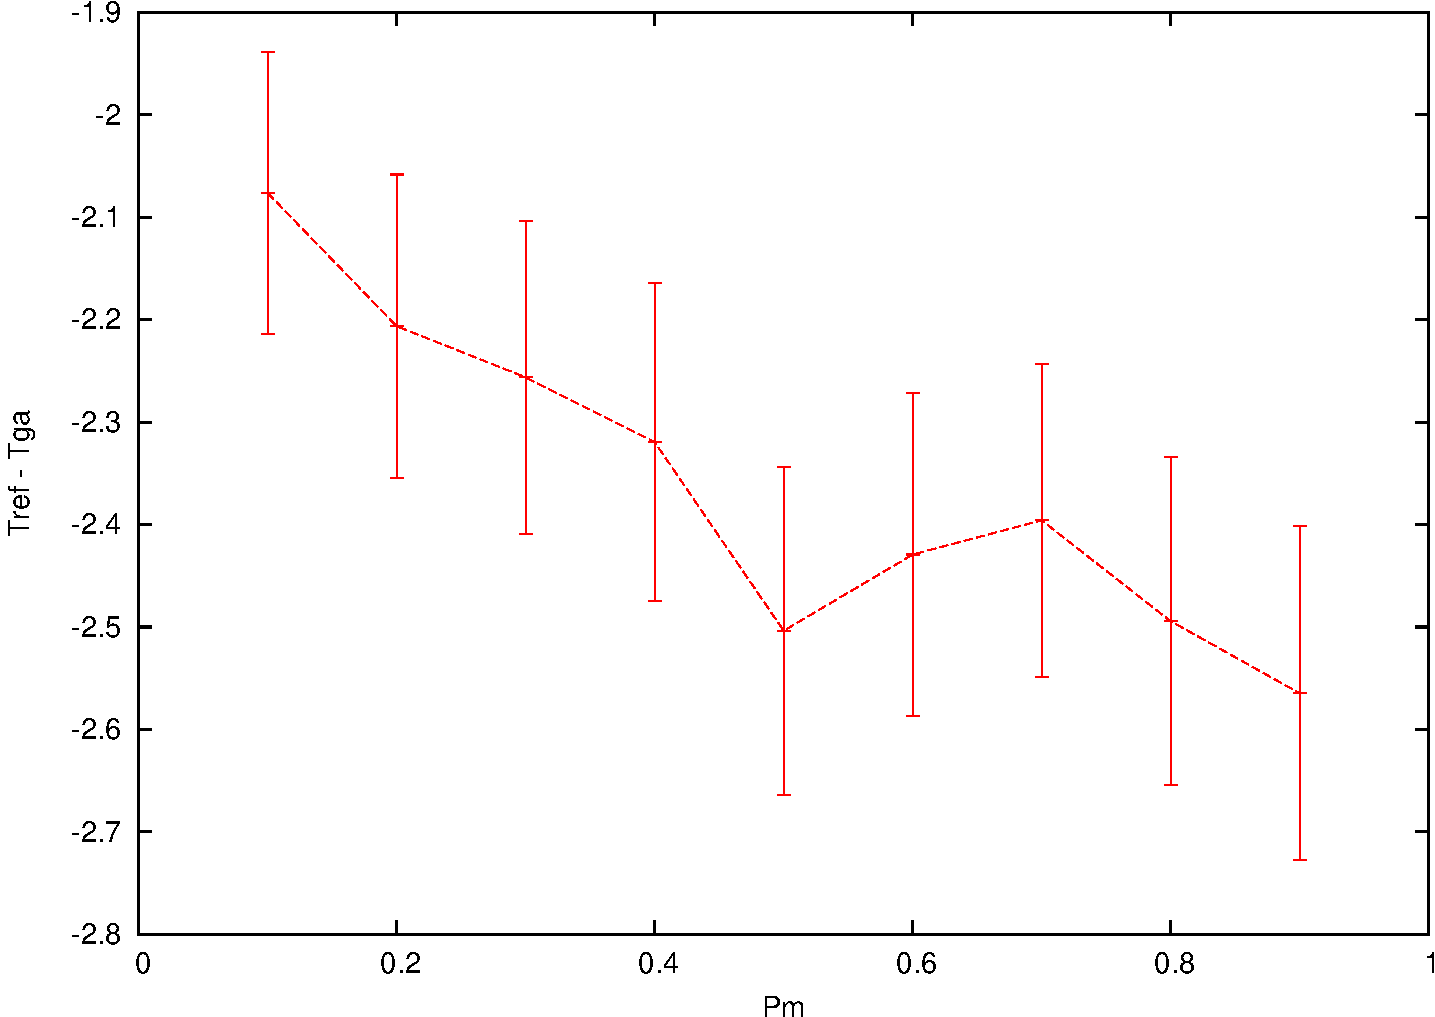
\includegraphics[width=\textwidth]{results_m_diff.pdf}
\caption{Evolution of $T_{ref}-T_{GA}$ for different $P_m$ values.}
\label{fig:evol_m_diff}
\end{subfigure}
~
\begin{subfigure}[b]{0.45\textwidth}
\centering
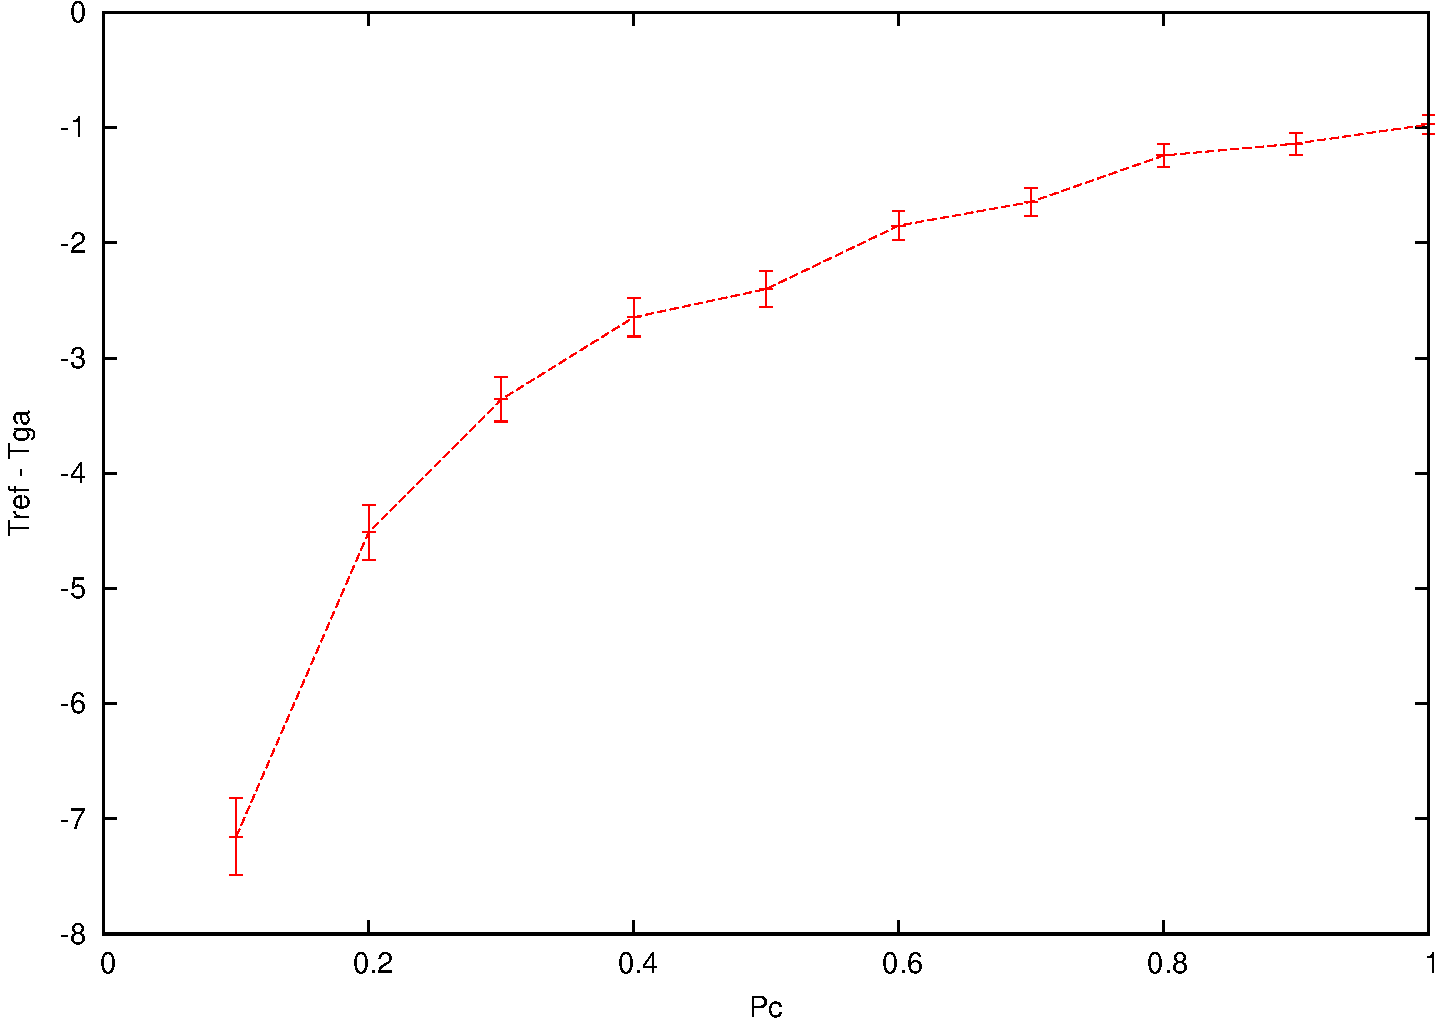
\includegraphics[width=\textwidth]{results_c_diff.pdf}
\caption{Evolution of $T_{ref}-T_{GA}$ for different $P_c$ values.}
\label{fig:evol_c_diff}
\end{subfigure}
\\
\begin{subfigure}[b]{0.45\textwidth}
\centering
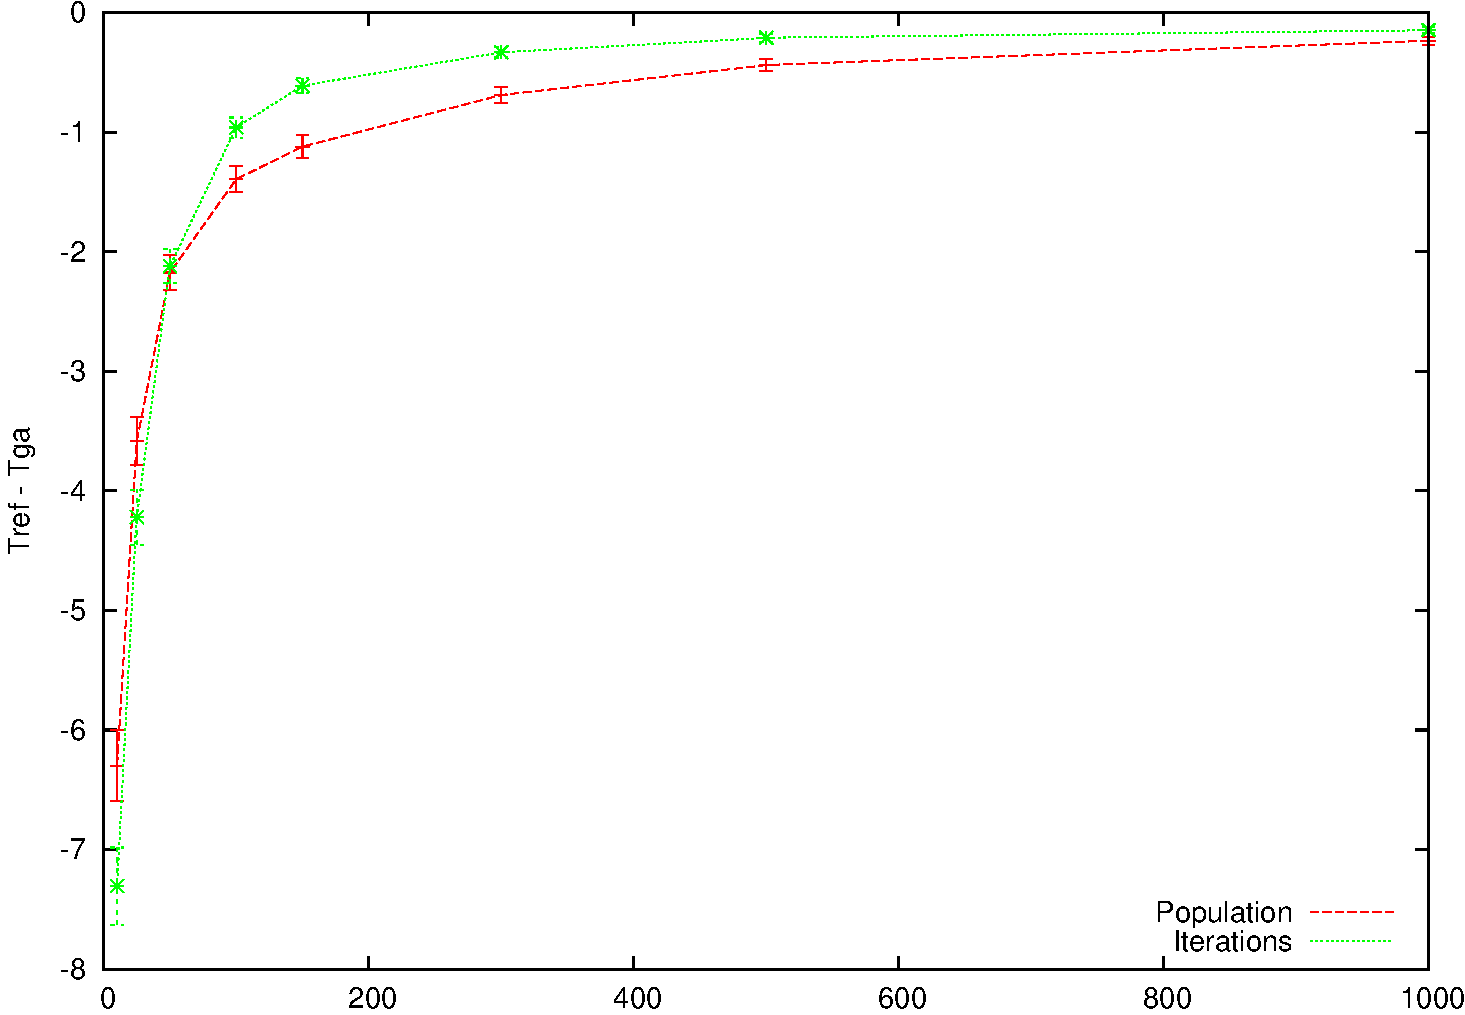
\includegraphics[width=\textwidth]{results_pop_it_diff.pdf}
\caption{Evolution of $T_{ref}-T_{GA}$ for different polpulation sizes (red) and number of iterations (green).}
\label{fig:evol_pop_it_diff}
\end{subfigure}
~
\begin{subfigure}[b]{0.45\textwidth}
\centering
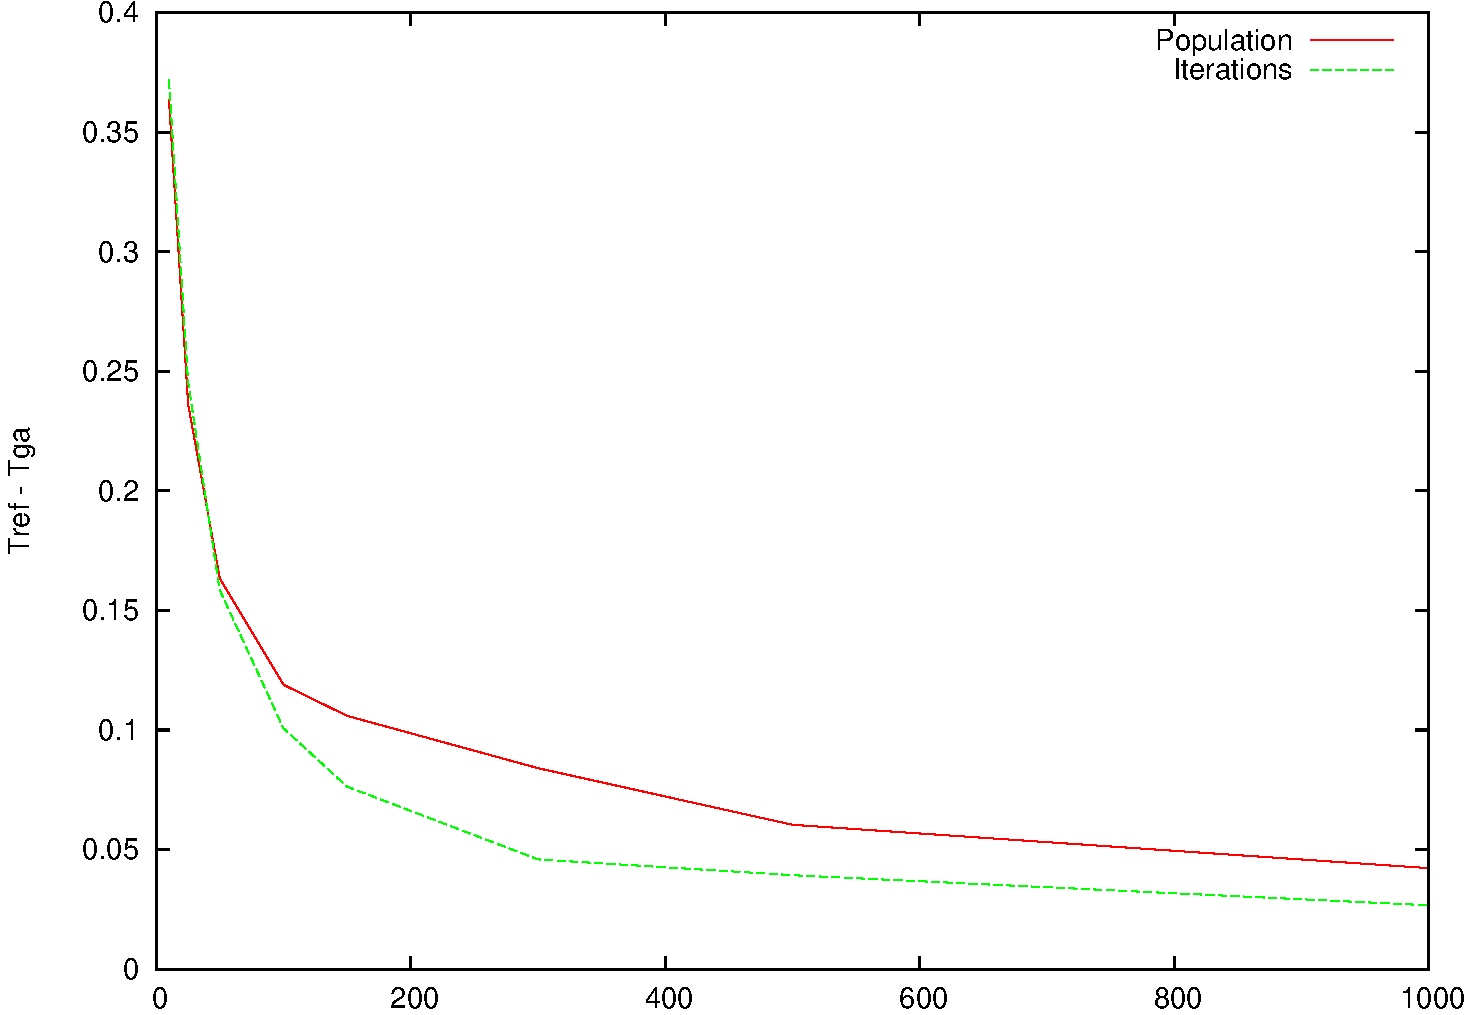
\includegraphics[width=\textwidth]{results_pop_it_worse.pdf}
\caption{Evolution of $P(T_{GA} > T_{ref})$ for different polpulation sizes (red) and number of iterations (green).}
\label{fig:evol_pop_it_worse}
\end{subfigure}
\caption{Performance of the GA for different parameters values.}
\end{figure}

A finally evaluation of the small and large instances was done using the values for each parameter shown in table \ref{tab:optimal_params}.

\begin{table}[h]
\centering
\begin{tabular}{|c|c|}
\hline
Parameter & Value \\
\hline
Population &  50\\
Iterations & 1000\\
$P_c$ & 1.0\\
$P_m$ & 0.1\\
\hline
\end{tabular}
\caption{Parameters used for the final evaluation of the small and large instances.}
\label{tab:optimal_params}
\end{table}

\section{Conclusions}

\bibliographystyle{abbrv}
\bibliography{jsp-ga}
\end{document}